\documentclass{standalone}
\usepackage{tikz}
\usetikzlibrary{patterns, positioning}


\begin{document}
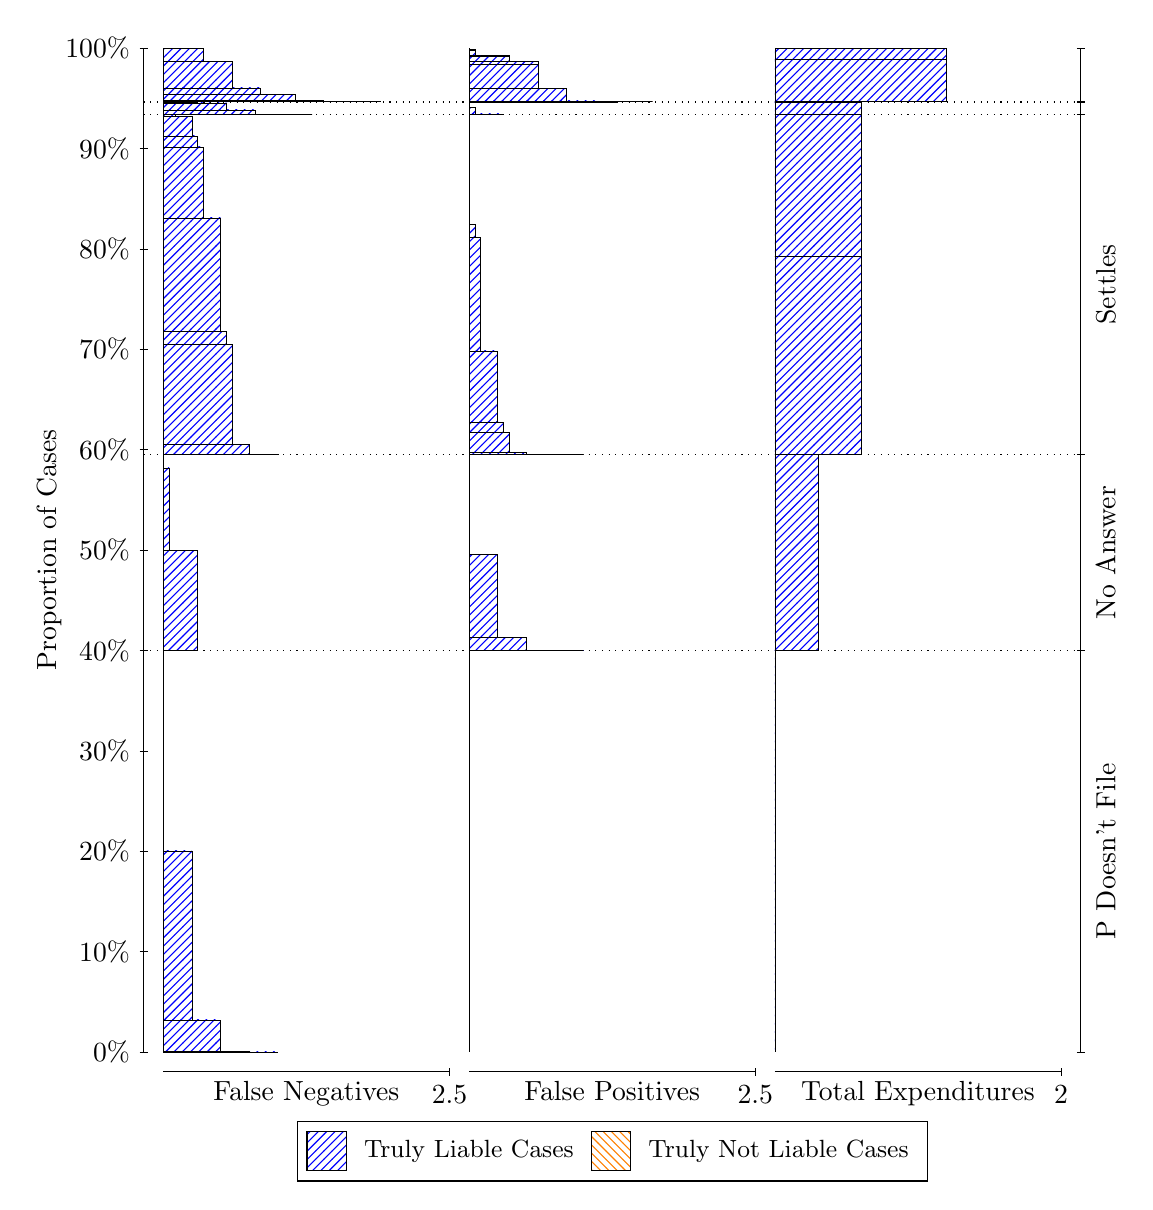
\begin{tikzpicture}
\draw[black, very thin] (1.5,1.75) -- (1.5,14.5);
\node[rotate=90, text=black, anchor=center] at (0.3, 8.125) {Proportion of Cases};
\draw[black, very thin] (1.45,1.75) -- (1.55,1.75);
\node[text=black, anchor=east] at (1.45, 1.75) {0\%};
\draw[black, very thin] (1.45,3.025) -- (1.55,3.025);
\node[text=black, anchor=east] at (1.45, 3.025) {10\%};
\draw[black, very thin] (1.45,4.3) -- (1.55,4.3);
\node[text=black, anchor=east] at (1.45, 4.3) {20\%};
\draw[black, very thin] (1.45,5.575) -- (1.55,5.575);
\node[text=black, anchor=east] at (1.45, 5.575) {30\%};
\draw[black, very thin] (1.45,6.85) -- (1.55,6.85);
\node[text=black, anchor=east] at (1.45, 6.85) {40\%};
\draw[black, very thin] (1.45,8.125) -- (1.55,8.125);
\node[text=black, anchor=east] at (1.45, 8.125) {50\%};
\draw[black, very thin] (1.45,9.4) -- (1.55,9.4);
\node[text=black, anchor=east] at (1.45, 9.4) {60\%};
\draw[black, very thin] (1.45,10.675) -- (1.55,10.675);
\node[text=black, anchor=east] at (1.45, 10.675) {70\%};
\draw[black, very thin] (1.45,11.95) -- (1.55,11.95);
\node[text=black, anchor=east] at (1.45, 11.95) {80\%};
\draw[black, very thin] (1.45,13.225) -- (1.55,13.225);
\node[text=black, anchor=east] at (1.45, 13.225) {90\%};
\draw[black, very thin] (1.45,14.5) -- (1.55,14.5);
\node[text=black, anchor=east] at (1.45, 14.5) {100\%};

\draw[black, very thin] (13.4,1.75) -- (13.4,14.5);
\draw[black, very thin] (13.35,1.75) -- (13.45,1.75);
\node[anchor=west] at (13.35, 1.75) {};
\draw[black, very thin] (13.35,6.8489) -- (13.45,6.8489);
\node[anchor=west] at (13.35, 6.8489) {};
\draw[black, very thin] (13.35,9.3359) -- (13.45,9.3359);
\node[anchor=west] at (13.35, 9.3359) {};
\draw[black, very thin] (13.35,13.661) -- (13.45,13.661);
\node[anchor=west] at (13.35, 13.661) {};
\draw[black, very thin] (13.35,13.805) -- (13.45,13.805);
\node[anchor=west] at (13.35, 13.805) {};
\draw[black, very thin] (13.35,13.821) -- (13.45,13.821);
\node[anchor=west] at (13.35, 13.821) {};
\draw[black, very thin] (13.35,14.5) -- (13.45,14.5);
\node[anchor=west] at (13.35, 14.5) {};

\draw[black, very thin, pattern color=blue, pattern=north east lines] (1.75,1.75) rectangle (3.2033,1.75);
\draw[black, very thin, pattern color=blue, pattern=north east lines] (1.75,1.75) rectangle (2.84,1.7534);
\draw[black, very thin, pattern color=blue, pattern=north east lines] (1.75,1.7534) rectangle (2.4767,2.158);
\draw[black, very thin, pattern color=blue, pattern=north east lines] (1.75,2.158) rectangle (2.1133,4.3029);
\draw[black, very thin, pattern color=orange, pattern=north west lines] (1.75,4.3029) rectangle (1.75,4.3029);
\draw[black, very thin, pattern color=blue, pattern=north east lines] (1.75,4.3029) rectangle (1.75,6.8489);
\draw[black, very thin, pattern color=blue, pattern=north east lines] (1.75,6.8489) rectangle (2.186,8.1167);
\draw[black, very thin, pattern color=blue, pattern=north east lines] (1.75,8.1167) rectangle (1.8227,9.169);
\draw[black, very thin, pattern color=orange, pattern=north west lines] (1.75,9.169) rectangle (1.75,9.169);
\draw[black, very thin, pattern color=blue, pattern=north east lines] (1.75,9.169) rectangle (1.75,9.3359);
\draw[black, very thin, pattern color=blue, pattern=north east lines] (1.75,9.3359) rectangle (3.2033,9.3364);
\draw[black, very thin, pattern color=blue, pattern=north east lines] (1.75,9.3364) rectangle (2.9127,9.3385);
\draw[black, very thin, pattern color=blue, pattern=north east lines] (1.75,9.3385) rectangle (2.84,9.4663);
\draw[black, very thin, pattern color=blue, pattern=north east lines] (1.75,9.4663) rectangle (2.622,10.737);
\draw[black, very thin, pattern color=blue, pattern=north east lines] (1.75,10.737) rectangle (2.5493,10.906);
\draw[black, very thin, pattern color=blue, pattern=north east lines] (1.75,10.906) rectangle (2.4767,12.343);
\draw[black, very thin, pattern color=blue, pattern=north east lines] (1.75,12.343) rectangle (2.2587,13.245);
\draw[black, very thin, pattern color=blue, pattern=north east lines] (1.75,13.245) rectangle (2.186,13.383);
\draw[black, very thin, pattern color=blue, pattern=north east lines] (1.75,13.383) rectangle (2.1133,13.629);
\draw[black, very thin, pattern color=blue, pattern=north east lines] (1.75,13.629) rectangle (1.8953,13.661);
\draw[black, very thin, pattern color=blue, pattern=north east lines] (1.75,13.661) rectangle (1.8227,13.661);
\draw[black, very thin, pattern color=orange, pattern=north west lines] (1.75,13.661) rectangle (1.75,13.661);
\draw[black, very thin, pattern color=blue, pattern=north east lines] (1.75,13.661) rectangle (1.75,13.661);
\draw[black, very thin, pattern color=blue, pattern=north east lines] (1.75,13.661) rectangle (3.6393,13.661);
\draw[black, very thin, pattern color=blue, pattern=north east lines] (1.75,13.661) rectangle (3.276,13.662);
\draw[black, very thin, pattern color=blue, pattern=north east lines] (1.75,13.662) rectangle (2.9127,13.715);
\draw[black, very thin, pattern color=blue, pattern=north east lines] (1.75,13.715) rectangle (2.5493,13.803);
\draw[black, very thin, pattern color=blue, pattern=north east lines] (1.75,13.803) rectangle (2.186,13.805);
\draw[black, very thin, pattern color=orange, pattern=north west lines] (1.75,13.805) rectangle (1.75,13.805);
\draw[black, very thin, pattern color=blue, pattern=north east lines] (1.75,13.805) rectangle (2.186,13.81);
\draw[black, very thin, pattern color=blue, pattern=north east lines] (1.75,13.81) rectangle (1.8227,13.82);
\draw[black, very thin, pattern color=orange, pattern=north west lines] (1.75,13.82) rectangle (1.75,13.82);
\draw[black, very thin, pattern color=blue, pattern=north east lines] (1.75,13.82) rectangle (1.75,13.821);
\draw[black, very thin, pattern color=blue, pattern=north east lines] (1.75,13.821) rectangle (4.5113,13.821);
\draw[black, very thin, pattern color=blue, pattern=north east lines] (1.75,13.821) rectangle (4.148,13.821);
\draw[black, very thin, pattern color=blue, pattern=north east lines] (1.75,13.821) rectangle (3.7847,13.834);
\draw[black, very thin, pattern color=blue, pattern=north east lines] (1.75,13.834) rectangle (3.712,13.834);
\draw[black, very thin, pattern color=blue, pattern=north east lines] (1.75,13.834) rectangle (3.4213,13.909);
\draw[black, very thin, pattern color=blue, pattern=north east lines] (1.75,13.909) rectangle (3.3487,13.91);
\draw[black, very thin, pattern color=blue, pattern=north east lines] (1.75,13.91) rectangle (3.058,13.911);
\draw[black, very thin, pattern color=blue, pattern=north east lines] (1.75,13.911) rectangle (2.9853,13.994);
\draw[black, very thin, pattern color=blue, pattern=north east lines] (1.75,13.994) rectangle (2.6947,13.994);
\draw[black, very thin, pattern color=blue, pattern=north east lines] (1.75,13.994) rectangle (2.622,14.334);
\draw[black, very thin, pattern color=blue, pattern=north east lines] (1.75,14.334) rectangle (2.2587,14.491);
\draw[black, very thin, pattern color=blue, pattern=north east lines] (1.75,14.491) rectangle (1.8953,14.5);
\draw[black, very thin, pattern color=orange, pattern=north west lines] (1.75,14.5) rectangle (1.75,14.5);
\draw[black, very thin, pattern color=blue, pattern=north east lines] (1.75,14.5) rectangle (1.75,14.5);
\draw[black, very thin, pattern color=orange, pattern=north west lines] (5.6333,1.75) rectangle (5.6333,1.75);
\draw[black, very thin, pattern color=blue, pattern=north east lines] (5.6333,1.75) rectangle (5.6333,6.8489);
\draw[black, very thin, pattern color=orange, pattern=north west lines] (5.6333,6.8489) rectangle (7.0867,6.8489);
\draw[black, very thin, pattern color=blue, pattern=north east lines] (5.6333,6.8489) rectangle (7.0867,6.8489);
\draw[black, very thin, pattern color=blue, pattern=north east lines] (5.6333,6.8489) rectangle (6.7233,6.8491);
\draw[black, very thin, pattern color=blue, pattern=north east lines] (5.6333,6.8491) rectangle (6.36,7.0157);
\draw[black, very thin, pattern color=blue, pattern=north east lines] (5.6333,7.0157) rectangle (5.9967,8.0681);
\draw[black, very thin, pattern color=blue, pattern=north east lines] (5.6333,8.0681) rectangle (5.6333,9.3359);
\draw[black, very thin, pattern color=orange, pattern=north west lines] (5.6333,9.3359) rectangle (7.0867,9.3359);
\draw[black, very thin, pattern color=blue, pattern=north east lines] (5.6333,9.3359) rectangle (7.0867,9.3359);
\draw[black, very thin, pattern color=orange, pattern=north west lines] (5.6333,9.3359) rectangle (6.796,9.3359);
\draw[black, very thin, pattern color=blue, pattern=north east lines] (5.6333,9.3359) rectangle (6.796,9.3359);
\draw[black, very thin, pattern color=blue, pattern=north east lines] (5.6333,9.3359) rectangle (6.7233,9.3359);
\draw[black, very thin, pattern color=orange, pattern=north west lines] (5.6333,9.3359) rectangle (6.5053,9.3359);
\draw[black, very thin, pattern color=blue, pattern=north east lines] (5.6333,9.3359) rectangle (6.5053,9.3364);
\draw[black, very thin, pattern color=blue, pattern=north east lines] (5.6333,9.3364) rectangle (6.4327,9.3367);
\draw[black, very thin, pattern color=blue, pattern=north east lines] (5.6333,9.3367) rectangle (6.36,9.3688);
\draw[black, very thin, pattern color=blue, pattern=north east lines] (5.6333,9.3688) rectangle (6.142,9.6142);
\draw[black, very thin, pattern color=blue, pattern=north east lines] (5.6333,9.6142) rectangle (6.0693,9.7523);
\draw[black, very thin, pattern color=blue, pattern=north east lines] (5.6333,9.7523) rectangle (5.9967,10.654);
\draw[black, very thin, pattern color=blue, pattern=north east lines] (5.6333,10.654) rectangle (5.7787,12.091);
\draw[black, very thin, pattern color=blue, pattern=north east lines] (5.6333,12.091) rectangle (5.706,12.26);
\draw[black, very thin, pattern color=blue, pattern=north east lines] (5.6333,12.26) rectangle (5.6333,13.661);
\draw[black, very thin, pattern color=orange, pattern=north west lines] (5.6333,13.661) rectangle (6.0693,13.661);
\draw[black, very thin, pattern color=blue, pattern=north east lines] (5.6333,13.661) rectangle (6.0693,13.664);
\draw[black, very thin, pattern color=blue, pattern=north east lines] (5.6333,13.664) rectangle (5.706,13.751);
\draw[black, very thin, pattern color=blue, pattern=north east lines] (5.6333,13.751) rectangle (5.6333,13.805);
\draw[black, very thin, pattern color=orange, pattern=north west lines] (5.6333,13.805) rectangle (7.5227,13.805);
\draw[black, very thin, pattern color=blue, pattern=north east lines] (5.6333,13.805) rectangle (7.5227,13.805);
\draw[black, very thin, pattern color=blue, pattern=north east lines] (5.6333,13.805) rectangle (7.1593,13.805);
\draw[black, very thin, pattern color=blue, pattern=north east lines] (5.6333,13.805) rectangle (6.796,13.805);
\draw[black, very thin, pattern color=blue, pattern=north east lines] (5.6333,13.805) rectangle (6.4327,13.816);
\draw[black, very thin, pattern color=blue, pattern=north east lines] (5.6333,13.816) rectangle (6.0693,13.821);
\draw[black, very thin, pattern color=orange, pattern=north west lines] (5.6333,13.821) rectangle (7.9587,13.821);
\draw[black, very thin, pattern color=blue, pattern=north east lines] (5.6333,13.821) rectangle (7.9587,13.821);
\draw[black, very thin, pattern color=orange, pattern=north west lines] (5.6333,13.821) rectangle (7.5953,13.821);
\draw[black, very thin, pattern color=blue, pattern=north east lines] (5.6333,13.821) rectangle (7.5953,13.821);
\draw[black, very thin, pattern color=orange, pattern=north west lines] (5.6333,13.821) rectangle (7.232,13.821);
\draw[black, very thin, pattern color=blue, pattern=north east lines] (5.6333,13.821) rectangle (7.232,13.829);
\draw[black, very thin, pattern color=blue, pattern=north east lines] (5.6333,13.829) rectangle (6.8687,13.986);
\draw[black, very thin, pattern color=orange, pattern=north west lines] (5.6333,13.986) rectangle (6.8687,13.986);
\draw[black, very thin, pattern color=blue, pattern=north east lines] (5.6333,13.986) rectangle (6.8687,13.987);
\draw[black, very thin, pattern color=blue, pattern=north east lines] (5.6333,13.987) rectangle (6.5053,14.291);
\draw[black, very thin, pattern color=blue, pattern=north east lines] (5.6333,14.291) rectangle (6.5053,14.326);
\draw[black, very thin, pattern color=orange, pattern=north west lines] (5.6333,14.326) rectangle (6.4327,14.326);
\draw[black, very thin, pattern color=blue, pattern=north east lines] (5.6333,14.326) rectangle (6.4327,14.326);
\draw[black, very thin, pattern color=blue, pattern=north east lines] (5.6333,14.326) rectangle (6.142,14.394);
\draw[black, very thin, pattern color=blue, pattern=north east lines] (5.6333,14.394) rectangle (6.142,14.409);
\draw[black, very thin, pattern color=blue, pattern=north east lines] (5.6333,14.409) rectangle (6.0693,14.41);
\draw[black, very thin, pattern color=orange, pattern=north west lines] (5.6333,14.41) rectangle (6.0693,14.41);
\draw[black, very thin, pattern color=blue, pattern=north east lines] (5.6333,14.41) rectangle (6.0693,14.411);
\draw[black, very thin, pattern color=blue, pattern=north east lines] (5.6333,14.411) rectangle (5.7787,14.411);
\draw[black, very thin, pattern color=blue, pattern=north east lines] (5.6333,14.411) rectangle (5.7787,14.411);
\draw[black, very thin, pattern color=blue, pattern=north east lines] (5.6333,14.411) rectangle (5.706,14.47);
\draw[black, very thin, pattern color=blue, pattern=north east lines] (5.6333,14.47) rectangle (5.706,14.486);
\draw[black, very thin, pattern color=blue, pattern=north east lines] (5.6333,14.486) rectangle (5.6333,14.5);
\draw[black, very thin, pattern color=orange, pattern=north west lines] (9.5167,1.75) rectangle (9.5167,1.75);
\draw[black, very thin, pattern color=blue, pattern=north east lines] (9.5167,1.75) rectangle (9.5167,6.8489);
\draw[black, very thin, pattern color=orange, pattern=north west lines] (9.5167,6.8489) rectangle (10.062,6.8489);
\draw[black, very thin, pattern color=blue, pattern=north east lines] (9.5167,6.8489) rectangle (10.062,9.3359);
\draw[black, very thin, pattern color=orange, pattern=north west lines] (9.5167,9.3359) rectangle (10.607,9.3359);
\draw[black, very thin, pattern color=blue, pattern=north east lines] (9.5167,9.3359) rectangle (10.607,11.85);
\draw[black, very thin, pattern color=orange, pattern=north west lines] (9.5167,11.85) rectangle (10.607,11.85);
\draw[black, very thin, pattern color=blue, pattern=north east lines] (9.5167,11.85) rectangle (10.607,13.661);
\draw[black, very thin, pattern color=orange, pattern=north west lines] (9.5167,13.661) rectangle (10.607,13.661);
\draw[black, very thin, pattern color=blue, pattern=north east lines] (9.5167,13.661) rectangle (10.607,13.805);
\draw[black, very thin, pattern color=orange, pattern=north west lines] (9.5167,13.805) rectangle (10.607,13.805);
\draw[black, very thin, pattern color=blue, pattern=north east lines] (9.5167,13.805) rectangle (10.607,13.821);
\draw[black, very thin, pattern color=orange, pattern=north west lines] (9.5167,13.821) rectangle (11.697,13.821);
\draw[black, very thin, pattern color=blue, pattern=north east lines] (9.5167,13.821) rectangle (11.697,14.359);
\draw[black, very thin, pattern color=orange, pattern=north west lines] (9.5167,14.359) rectangle (11.697,14.359);
\draw[black, very thin, pattern color=blue, pattern=north east lines] (9.5167,14.359) rectangle (11.697,14.5);
\draw[black, dotted] (1.5,6.8489) -- (13.4,6.8489);
\draw[black, dotted] (1.5,9.3359) -- (13.4,9.3359);
\draw[black, dotted] (1.5,13.661) -- (13.4,13.661);
\draw[black, dotted] (1.5,13.805) -- (13.4,13.805);
\draw[black, dotted] (1.5,13.821) -- (13.4,13.821);
\draw[black, very thin] (1.75,1.5) -- (5.3833,1.5);
\node[text=black, anchor=north] at (3.5667, 1.5) {False Negatives};
\draw[black, very thin] (5.3833,1.45) -- (5.3833,1.55);
\node[text=black, anchor=north] at (5.3833, 1.45) {2.5};

\draw[black, very thin] (5.6333,1.5) -- (9.2667,1.5);
\node[text=black, anchor=north] at (7.45, 1.5) {False Positives};
\draw[black, very thin] (9.2667,1.45) -- (9.2667,1.55);
\node[text=black, anchor=north] at (9.2667, 1.45) {2.5};

\draw[black, very thin] (9.5167,1.5) -- (13.15,1.5);
\node[text=black, anchor=north] at (11.333, 1.5) {Total Expenditures};
\draw[black, very thin] (13.15,1.45) -- (13.15,1.55);
\node[text=black, anchor=north] at (13.15, 1.45) {2};

\node[text=black, centered, rotate=90] at (13.72, 4.2994) {P Doesn't File};
\node[text=black, centered, rotate=90] at (13.72, 8.0924) {No Answer};
\node[text=black, centered, rotate=90] at (13.72, 11.499) {Settles};




\draw (7.449999999999999,1.5) node[draw=none] (baseCoordinate) {};
\begin{scope}[align=center]
        \matrix[scale=0.5, draw=black, below=0.5cm of baseCoordinate, nodes={draw}, column sep=0.1cm]{
            \node[rectangle, draw, minimum width=0.5cm, minimum height=0.5cm, pattern color=blue, pattern=north east lines] {}; &
            \node[draw=none, font=\small, text=black] (B) {Truly Liable Cases}; &
            \node[rectangle, draw, minimum width=0.5cm, minimum height=0.5cm, pattern color=orange, pattern=north west lines] {}; &
            \node[draw=none, font=\small, text=black] (B) {Truly Not Liable Cases}; \\
            };
\end{scope}

\end{tikzpicture}
\end{document}